\documentclass[10pt,aspectratio=169]{ntuabeamer}
\usepackage{appendixnumberbeamer}

% --- Packages ---
\usepackage{amsmath, amssymb, amsthm, mathtools}
\usepackage{booktabs}
\usepackage{graphicx}
\usepackage{algorithm}
\usepackage{algpseudocode}
\usepackage{xcolor}
\usepackage{tikz}

% --- Custom Macros for Rigor ---
\newcommand{\R}{\mathbb{R}}
\newcommand{\E}{\mathbb{E}}
\newcommand{\prob}{P}
\newcommand{\K}{\mathcal{K}}
% One plain sentence closing a frame: what the audience should take away.
\newcommand{\takeaway}[1]{\par\vspace{0.7em}\textcolor{ntuablue}{\textbf{So} #1}\par}
\DeclareMathOperator*{\argmin}{arg\,min}
\DeclareMathOperator*{\infimum}{inf}

% --- Title Info ---
\title[Stochastic Methods]{Measures of Discrepancy for Distributions}
\author{NTUA School of Civil Engineering}


\graphicspath{{assets/}}
\begin{document}
	% --- Title Slide ---
	\begin{frame}
		\makepresentationtitle
	\end{frame}

	% --- TOC ---
	% ==============================================================================
	% SECTION 1: KERNEL DENSITY ESTIMATION
	% ==============================================================================
	\section{Estimating a Density (KDE)}
	\sectiondivider{Estimating a Density (KDE)}

	\begin{frame}{Estimating a Density from Samples}
\small
\[
 X_1,\ldots,X_n\overset{\mathrm{i.i.d.}}\sim f,\qquad f\text{ unknown}.
\]
\begin{itemize}
\item Independent observations share the same probability density $f$.
\item Goal: estimate its shape from samples.
\item A Normal fit can miss skewness, multiple peaks and heavy tails.
\item KDE estimates the density without choosing a parametric family.
\end{itemize}
\end{frame}

	\begin{frame}{The Idea: A Small Bump on Every Sample}
		\small
		A histogram counts samples per bin, so its look depends on where the bins start.
		A \textbf{kernel density estimate (KDE)} instead places a small smooth bump on every sample and adds the bumps up:
		where samples crowd together the bumps pile up high; where samples are rare the curve is low.

		\begin{figure}
			\centering
			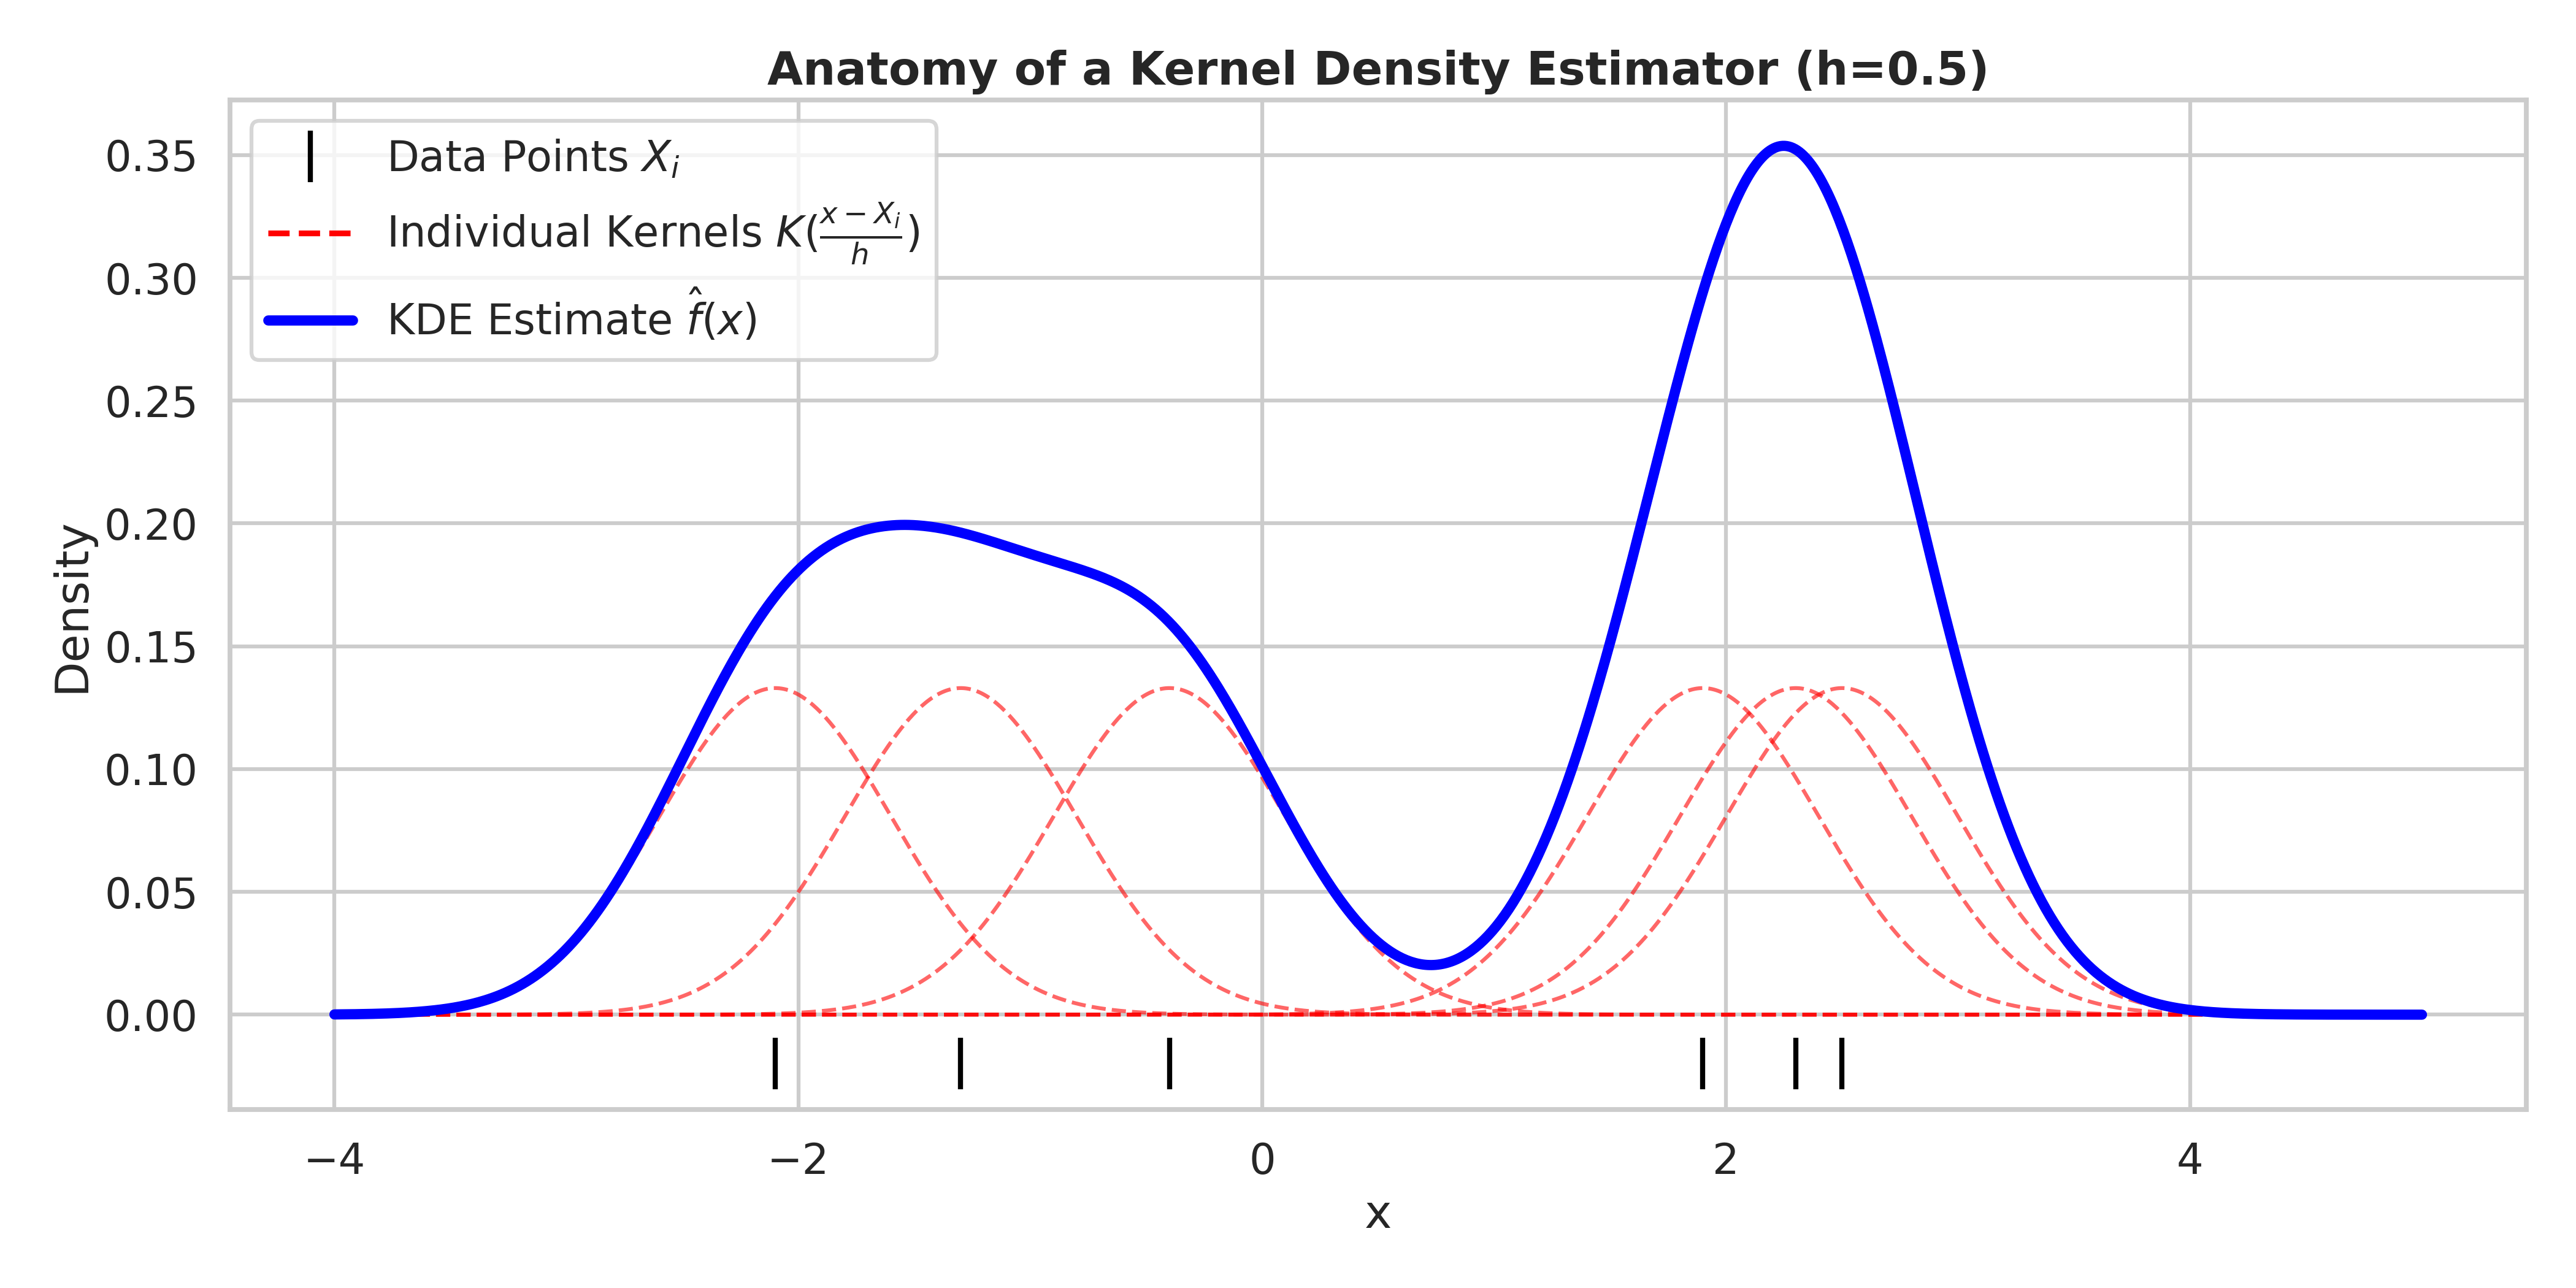
\includegraphics[width=0.55\textwidth]{kde_anatomy.png}
			\caption{\footnotesize Each observation $X_i$ (ticks) contributes one bump (dashed). The solid curve $\hat f$ is their normalized sum.}
		\end{figure}
		\takeaway{a KDE is ``a bump per sample, added up'': a smooth density built straight from the data.}
	\end{frame}

	\begin{frame}{The Estimator in Symbols}
\small
\begin{block}{Parzen--Rosenblatt estimator}
\[
 \widehat f_h(x)=\frac1{nh^d}\sum_{i=1}^n K\!\left(\frac{x-X_i}{h}\right).
\]
\end{block}
\begin{itemize}
\item $X_i\in\mathbb R^d$: independent samples from the same distribution.
\item $x\in\mathbb R^d$: evaluation point; $K$: centered, non-negative, unit-mass kernel.
\item $h>0$: bandwidth, controlling bump width.
\item $h^{-d}$ preserves each bump's mass; $1/n$ averages the bumps.
\end{itemize}
\end{frame}

	\begin{frame}{What Counts as a Kernel?}
\small
\begin{align*}
 K(u)&\ge0 &&\text{non-negative density estimate},\\
 \int K(u)\,du&=1 &&\text{unit total mass},\\
 \int uK(u)\,du&=0 &&\text{centered bump (when the moment exists)}.
\end{align*}
\begin{itemize}
\item Non-negativity and unit mass make the KDE a density.
\item Centering avoids a systematic shift; symmetry ensures it when the first moment exists.
\item Kernel variance enters the error analysis in the appendix.
\end{itemize}
\end{frame}

	\begin{frame}{Common Kernels}
		\small
		\begin{table}[]
			\centering
			\renewcommand{\arraystretch}{1.9}
			\begin{tabular}{l l l}
				\toprule
				\textbf{Kernel} & \textbf{Function} $K(u)$ & \textbf{Support} \\
				\midrule
				Gaussian & $\displaystyle \frac{1}{\sqrt{2\pi}} \exp\left(-\frac{1}{2}u^2\right)$ & $u \in \mathbb{R}$ \\
				Epanechnikov & $\displaystyle \frac{3}{4}(1 - u^2)$ & $|u| \le 1$ \\
				Uniform & $\displaystyle \frac{1}{2}$ & $|u| \le 1$ \\
				Triangular & $\displaystyle (1 - |u|)$ & $|u| \le 1$ \\
				\bottomrule
			\end{tabular}
		\end{table}

		The Epanechnikov kernel has the smallest estimation error among non-negative kernels of the same width,
		but the Gaussian is only a few percent worse.

		\takeaway{the kernel shape hardly matters; the bandwidth $h$ matters far more.}
	\end{frame}

	\begin{frame}{The Bandwidth Dilemma}
\small
\begin{columns}[c]
\column{0.43\textwidth}
\[
 \widehat p_h(x)=\frac1{nh}\sum_{i=1}^n K\!\left(\frac{x-X_i}{h}\right).
\]
Small $h$: noisy spikes (high variance).\\[0.5em]
Large $h$: merged peaks (high bias).
\column{0.55\textwidth}
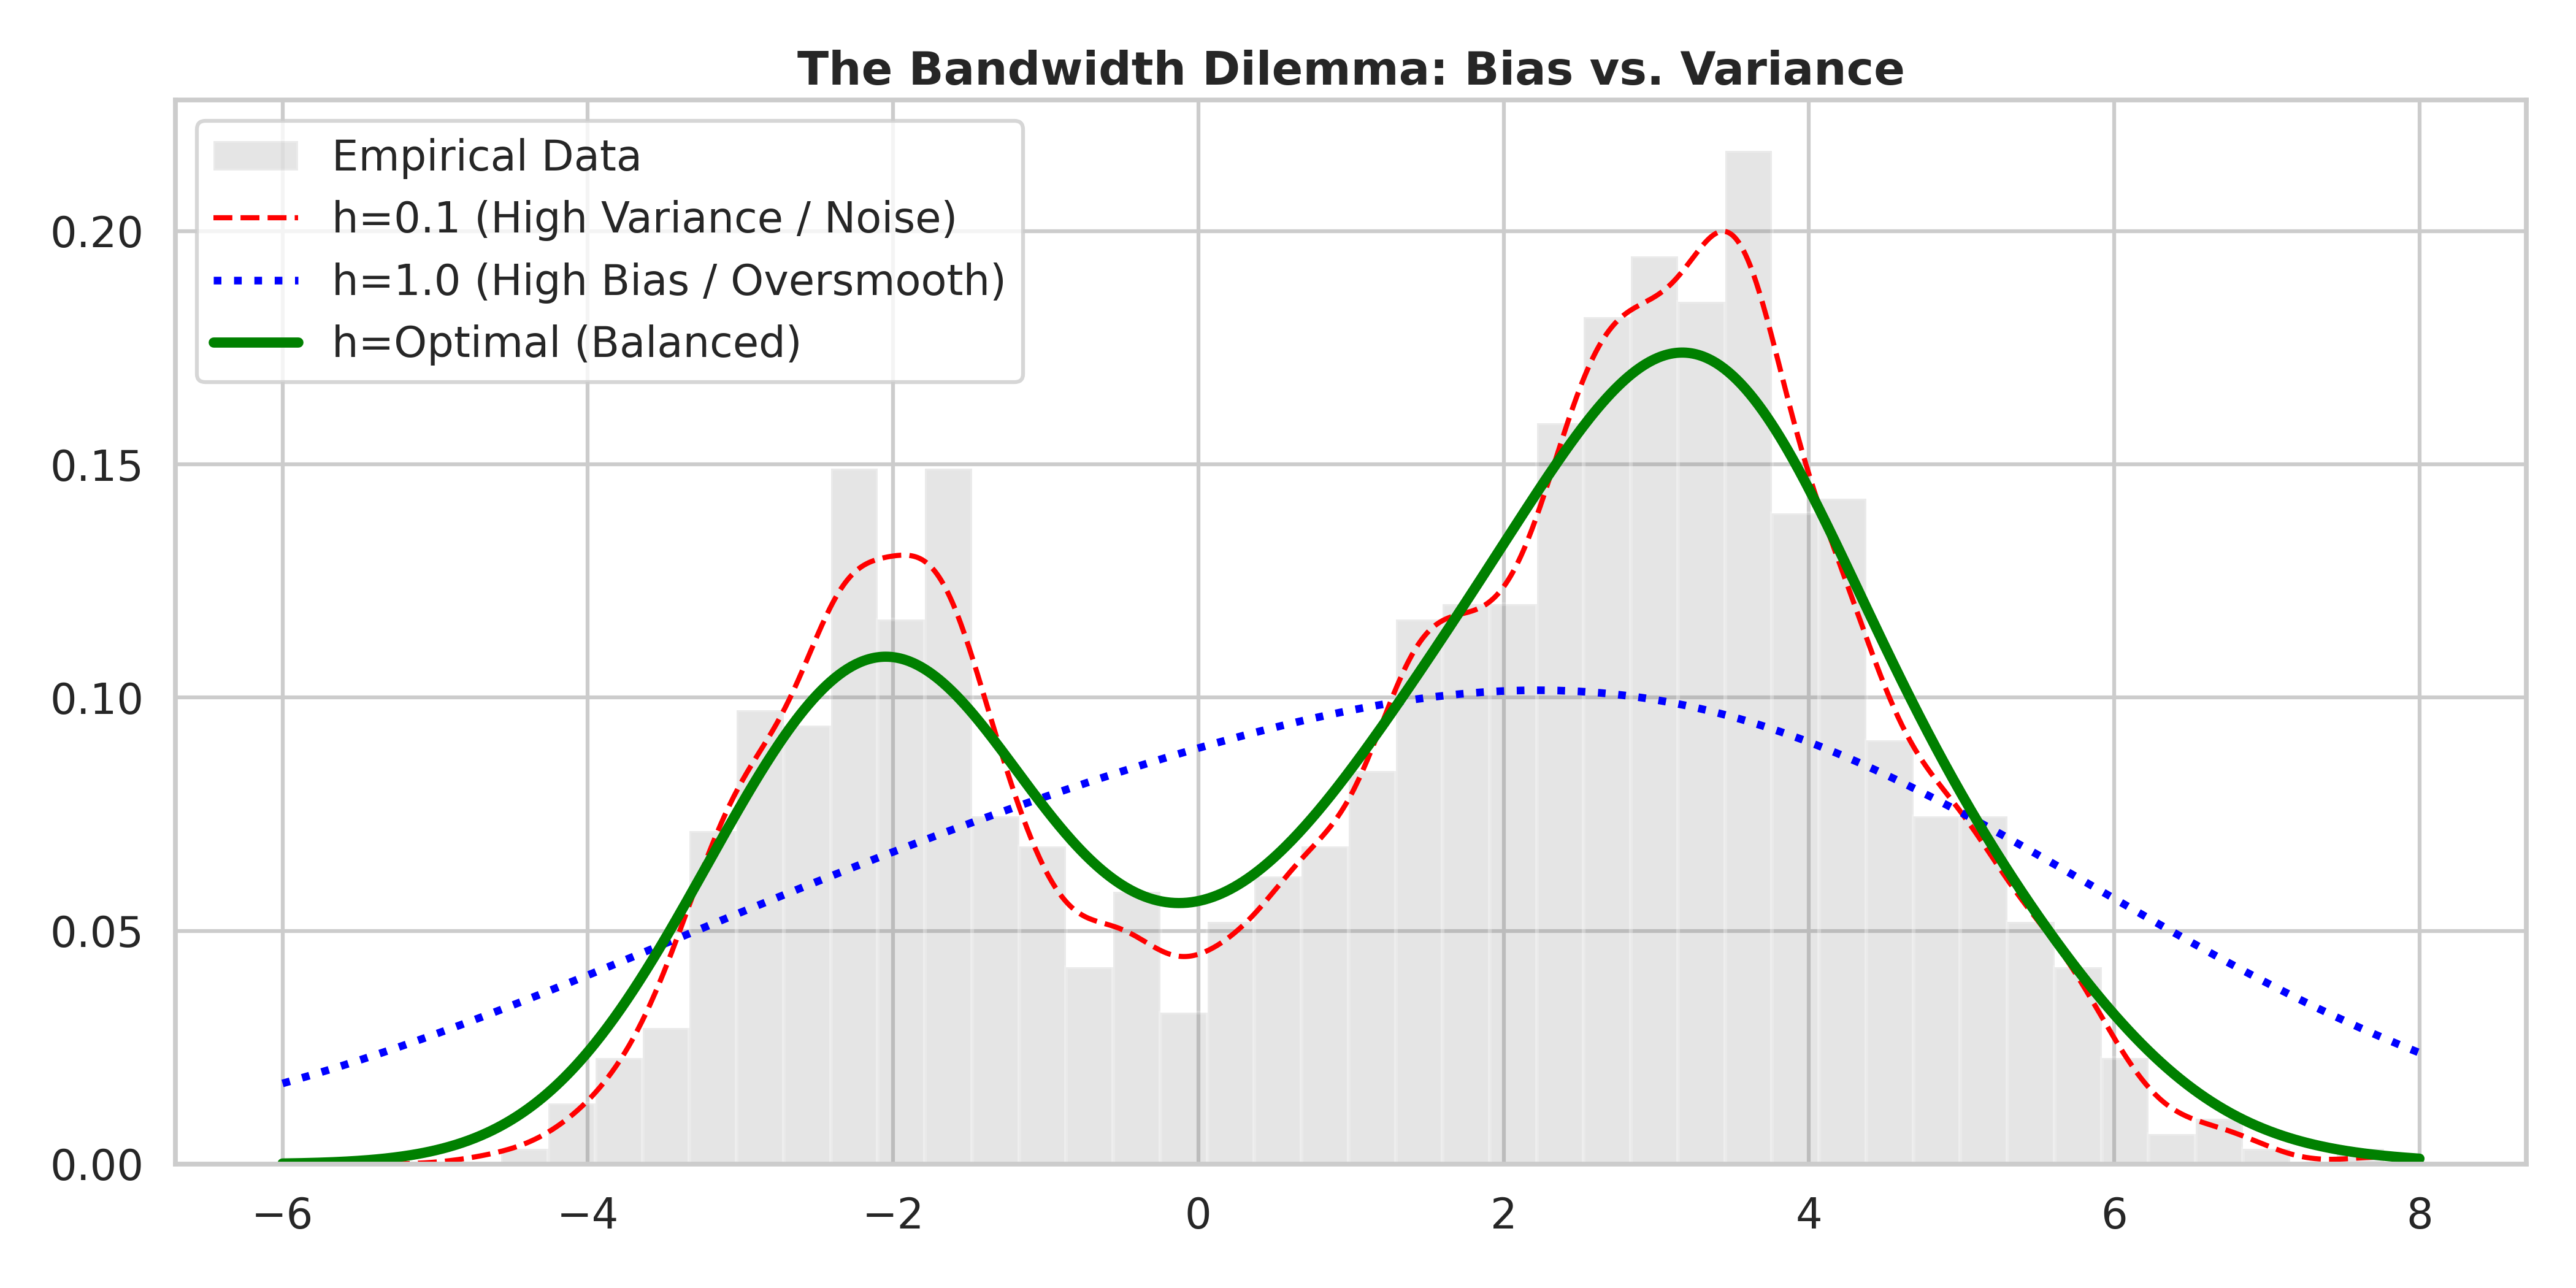
\includegraphics[width=\linewidth]{kde_bandwidths.png}
\end{columns}
\takeaway{the same samples give very different density estimates as $h$ changes.}
\end{frame}

	\begin{frame}{Why a Best Bandwidth Exists}
\small
For a smooth 1-D density and a second-order kernel,
\[
 \operatorname{AMISE}(h)=\underbrace{\frac{R(K)}{nh}}_{\text{variance}}
 +\underbrace{\frac{h^4\mu_2(K)^2R(f'')}{4}}_{\text{squared bias}},\qquad
 h_{\mathrm{opt}}\propto n^{-1/5}.
\]
\begin{itemize}
\item Wider bumps reduce sampling noise but blur peaks.
\item $R(g)=\int g^2$; $\mu_2(K)=\int u^2K(u)\,du$.
\item $100\times$ more data permits about $0.40\times$ the bandwidth.
\item The optimal constant depends on the unknown curvature of $f$.
\end{itemize}
\end{frame}

	\begin{frame}{Choosing $h$ in Practice}
\small
\textbf{Gaussian kernel, roughly Normal data: Silverman's rule}
\[
 h\approx1.06\,\widehat\sigma n^{-1/5}.
\]
\begin{itemize}
\item $\widehat\sigma$: sample standard deviation.
\item Example: $n=100$, $\widehat\sigma=2$ gives $h\approx0.84$.
\item Several peaks inflate $\widehat\sigma$; the rule can oversmooth.
\item Inspect the KDE; compare bandwidths or use least-squares cross-validation (appendix).
\end{itemize}
\end{frame}

	% ==============================================================================
	% SECTION 2: METRICS ON PROBABILITY SPACES
	% ==============================================================================
	\section{Comparing Two Distributions}
	\sectiondivider{Comparing Two Distributions}

	\begin{frame}{What Do We Want from a ``Distance'' Between Distributions?}
\small
\centering
\begin{tikzpicture}[x=0.8cm,y=0.65cm,>=stealth]
\foreach \y/\shift/\label in {4/0.5/Overlap,2/2/Disjoint,0/5/Far apart}{
 \node[anchor=east] at (-0.2,\y+0.5) {\label};
 \draw[->,gray] (0,\y)--(8,\y);
 \fill[ntuablue!35] (0.5,\y) rectangle (2,\y+1);
 \fill[orange!55,opacity=0.65] (0.5+\shift,\y) rectangle (2+\shift,\y+1);
}
\node[ntuablue] at (7.8,5) {$P$}; \node[orange!80!black] at (7.8,4.5) {$Q$};
\end{tikzpicture}
\par\raggedright
KL checks whether $Q$ covers $P$; JSD detects overlap but saturates once disjoint.
$W_1$ also measures the distance between their locations.
\end{frame}

	% --- KL Divergence ---
	\begin{frame}{Kullback--Leibler (KL) Divergence}
		\small
		\begin{block}{Definition (relative entropy)}
			$$ D_{KL}(P \| Q) = \int p(x) \log \frac{p(x)}{q(x)}\, dx = \E_{x \sim P}\!\left[\log \frac{p(x)}{q(x)}\right] $$
		\end{block}
		\begin{itemize}
			\item $\E_{x\sim P}[\cdot]$ is an average over samples drawn from $P$.
			\item $\log\frac{p}{q}$: how many times more likely $P$ finds a point than $Q$ does (on a log scale).
			\item So $D_{KL}$ is the extra ``surprise'' we suffer when we use $Q$ to describe data that really come from $P$.
			\item $D_{KL}\ge 0$, and $D_{KL}=0$ exactly when $P=Q$.
		\end{itemize}
		\takeaway{KL measures how badly $Q$ explains data from $P$.}
	\end{frame}

	\begin{frame}{KL Is Not Symmetric: A Numeric Check}
		\small
		Two coins: $P=(0.5,\,0.5)$ and $Q=(0.9,\,0.1)$ (probabilities of heads and tails).
		\begin{align*}
			D_{KL}(P\|Q) &= 0.5\ln\tfrac{0.5}{0.9}+0.5\ln\tfrac{0.5}{0.1} \approx 0.511,\\
			D_{KL}(Q\|P) &= 0.9\ln\tfrac{0.9}{0.5}+0.1\ln\tfrac{0.1}{0.5} \approx 0.368.
		\end{align*}
		The two directions give different numbers, so KL is a \emph{divergence}, not a distance in the usual sense (it also violates the triangle inequality).
		The direction matters: $D_{KL}(P\|Q)$ punishes $Q$ for missing outcomes that $P$ often produces.

		\takeaway{always say which distribution comes first; $D_{KL}(P\|Q)\neq D_{KL}(Q\|P)$.}
	\end{frame}

	\begin{frame}{KL Can Be Infinite}
\small
\[
 P(A)>0,\quad Q(A)=0\quad\Longrightarrow\quad D_{KL}(P\|Q)=\infty.
\]
\begin{itemize}
\item $Q$ must cover the support of $P$; coverage alone does not guarantee finite KL.
\item Disjoint supports give infinite KL regardless of their separation.
\item Near-zero estimated $q$ can produce unstable scores.
\end{itemize}
\[
 P=(0.5,0.5),\quad Q=(1,0):\qquad
 D_{KL}(P\|Q)=\infty,\quad D_{KL}(Q\|P)=\ln2.
\]
\end{frame}

	% --- Jensen-Shannon ---
	\begin{frame}{Jensen--Shannon Divergence (JSD)}
		\small
		\textbf{Idea:} compare both $P$ and $Q$ with their average, instead of with each other.
		The mixture $M=\tfrac12(P+Q)$ is positive wherever either one is, so no division by zero occurs.
		\begin{block}{Definition}
			$$ JSD(P \| Q) = \tfrac{1}{2} D_{KL}(P \| M) + \tfrac{1}{2} D_{KL}(Q \| M) $$
		\end{block}
		\textbf{Example} (the two coins): $M=(0.7,0.3)$, $D_{KL}(P\|M)\approx 0.087$, $D_{KL}(Q\|M)\approx 0.116$, so $JSD\approx 0.102$.

		\begin{itemize}
			\item \textbf{Symmetric:} $JSD(P\|Q)=JSD(Q\|P)$.
			\item \textbf{Bounded:} $0\le JSD\le\log 2\approx 0.693$ (natural log).
		\end{itemize}
		\takeaway{JSD is the symmetric, always-finite version of KL.}
	\end{frame}

	\begin{frame}{JSD Saturates for Non-Overlapping Distributions}
\small
\[
 \operatorname{supp}(P)\cap\operatorname{supp}(Q)=\varnothing
 \quad\Longrightarrow\quad JSD(P\|Q)=\log2.
\]
\begin{itemize}
\item Nearby and distant disjoint distributions receive the same maximum score.
\item Small moves preserving disjointness leave JSD unchanged.
\item This plateau can deprive a generator of a useful learning signal.
\item Near-disjoint distributions approach the plateau; KL may instead diverge.
\end{itemize}
\end{frame}

	% --- Optimal Transport ---
	\begin{frame}{Wasserstein Distance: The Idea}
\small
\centering
\begin{tikzpicture}[>=stealth,scale=1.4,transform shape]
\fill[ntuablue] (0,0) circle (4pt) node[below] {$P=\delta_0$};
\fill[orange] (6,0) circle (4pt) node[below] {$Q=\delta_a$};
\draw[->,thick] (0,0.5)--node[above] {move unit mass a distance $a$} (6,0.5);
\end{tikzpicture}
\[
 \text{transport cost}=\text{mass}\times\text{distance},\qquad W_1(\delta_0,\delta_a)=|a|.
\]
\raggedright
\begin{itemize}
\item Find the cheapest redistribution of $P$ into $Q$.
\item Preserve all mass; use the geometry of the underlying space.
\item Separation remains informative even for disjoint supports.
\end{itemize}
\end{frame}

	\begin{frame}{Wasserstein Distance: The Definition}
\small
For $p\ge1$ and distributions with finite $p$th moments,
\[
 W_p(P,Q)=\left(\inf_{\gamma\in\Pi(P,Q)}\int d(x,y)^p\,d\gamma(x,y)\right)^{1/p}.
\]
\begin{itemize}
\item $d(x,y)$: ground metric, such as Euclidean distance.
\item $\gamma$: transport plan assigning mass to source--destination pairs.
\item $\Pi(P,Q)$: plans whose marginals equal $P$ and $Q$.
\item Minimize transport cost, then take the $p$th root; $W_1$ uses cost proportional to distance.
\end{itemize}
\end{frame}

	\begin{frame}{Wasserstein Distance: A Picture}
		\small
		\begin{columns}
			\column{0.4\textwidth}
			\begin{figure}
				\centering
				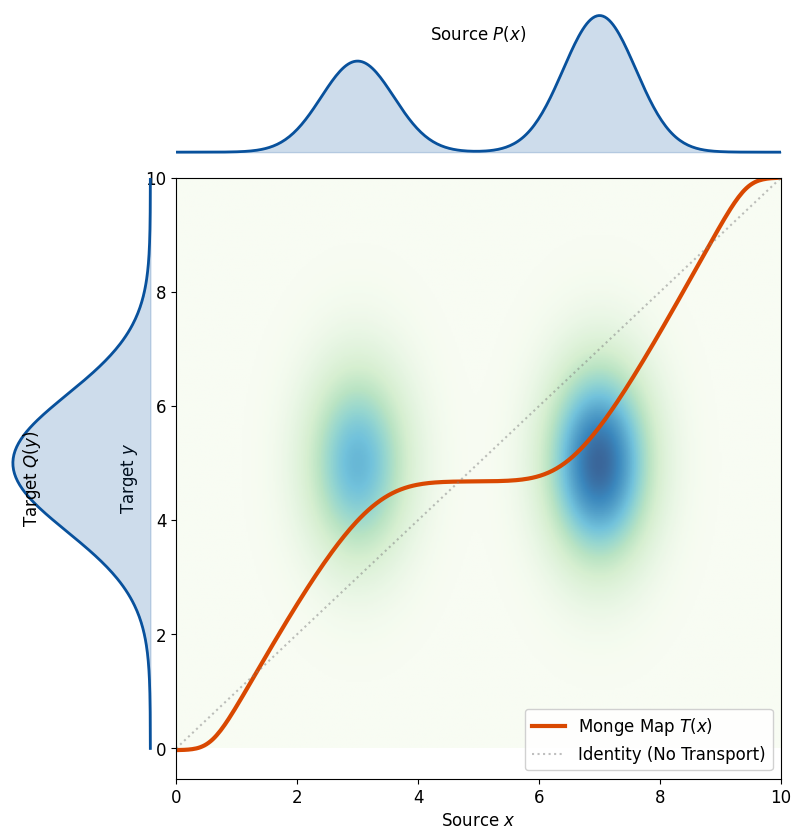
\includegraphics[width=\linewidth]{optimal-transport.png}
			\end{figure}
			\column{0.58\textwidth}
\[W_1(P,Q)=\inf_{\gamma\in\Pi(P,Q)}\int d(x,y)\,d\gamma(x,y).\]
			\begin{itemize}
				\item Top: source density $P(x)$. Left: target density $Q(y)$.
				\item The curve shows where the cheapest plan sends mass that starts at $x$.
				\item The shaded area shows where the plan puts its mass.
				\item The diagonal would mean ``nothing moves''.
			\end{itemize}
		\end{columns}
		\takeaway{the optimal plan moves mass as little as possible, never creating or destroying any.}
	\end{frame}

	\begin{frame}{The Same Shift, Three Answers}
		\small
		Take $P$ with all mass at $0$ and $Q$ with all mass at $a$ (idealized, sharply peaked distributions), and shift $Q$ farther away:

		\begin{table}[]
			\centering
			\renewcommand{\arraystretch}{1.3}
			\begin{tabular}{c c c c}
				\toprule
				shift $a$ & $D_{KL}(P\|Q)$ & $JSD$ & $W_1$ \\
				\midrule
				$1$ & $\infty$ & $\log 2\approx 0.69$ & $1$ \\
				$2$ & $\infty$ & $\log 2\approx 0.69$ & $2$ \\
				$5$ & $\infty$ & $\log 2\approx 0.69$ & $5$ \\
				\bottomrule
			\end{tabular}
		\end{table}
		For Gaussian densities with equal variance, KL grows quadratically with the shift; JSD approaches its bound. Smoothness alone does not imply finite KL.
		$W_1$ for a pure translation equals the size of the shift, $|a|$.

		\takeaway{only Wasserstein still reports how far apart two non-overlapping distributions are.}
	\end{frame}

	% ==============================================================================
	% SECTION 3: APPLICATIONS
	% ==============================================================================
	\section{Applications in ML Engineering}
	\sectiondivider{Applications in ML Engineering}

	\begin{frame}{Application 1: Drift Detection}
		\small
		\begin{columns}
			\column{0.4\textwidth}
			A deployed model sees data that slowly change. \textbf{Covariate shift}: the input distribution $P(X)$ changes while the relation $P(Y|X)$ stays the same.

			\vspace{0.8em}
			We compare a \emph{reference} sample (training data) with a \emph{current} sample (live data).
			When overlap vanishes, KL can diverge and JSD saturates.

			\column{0.6\textwidth}
			\begin{figure}
				\centering
				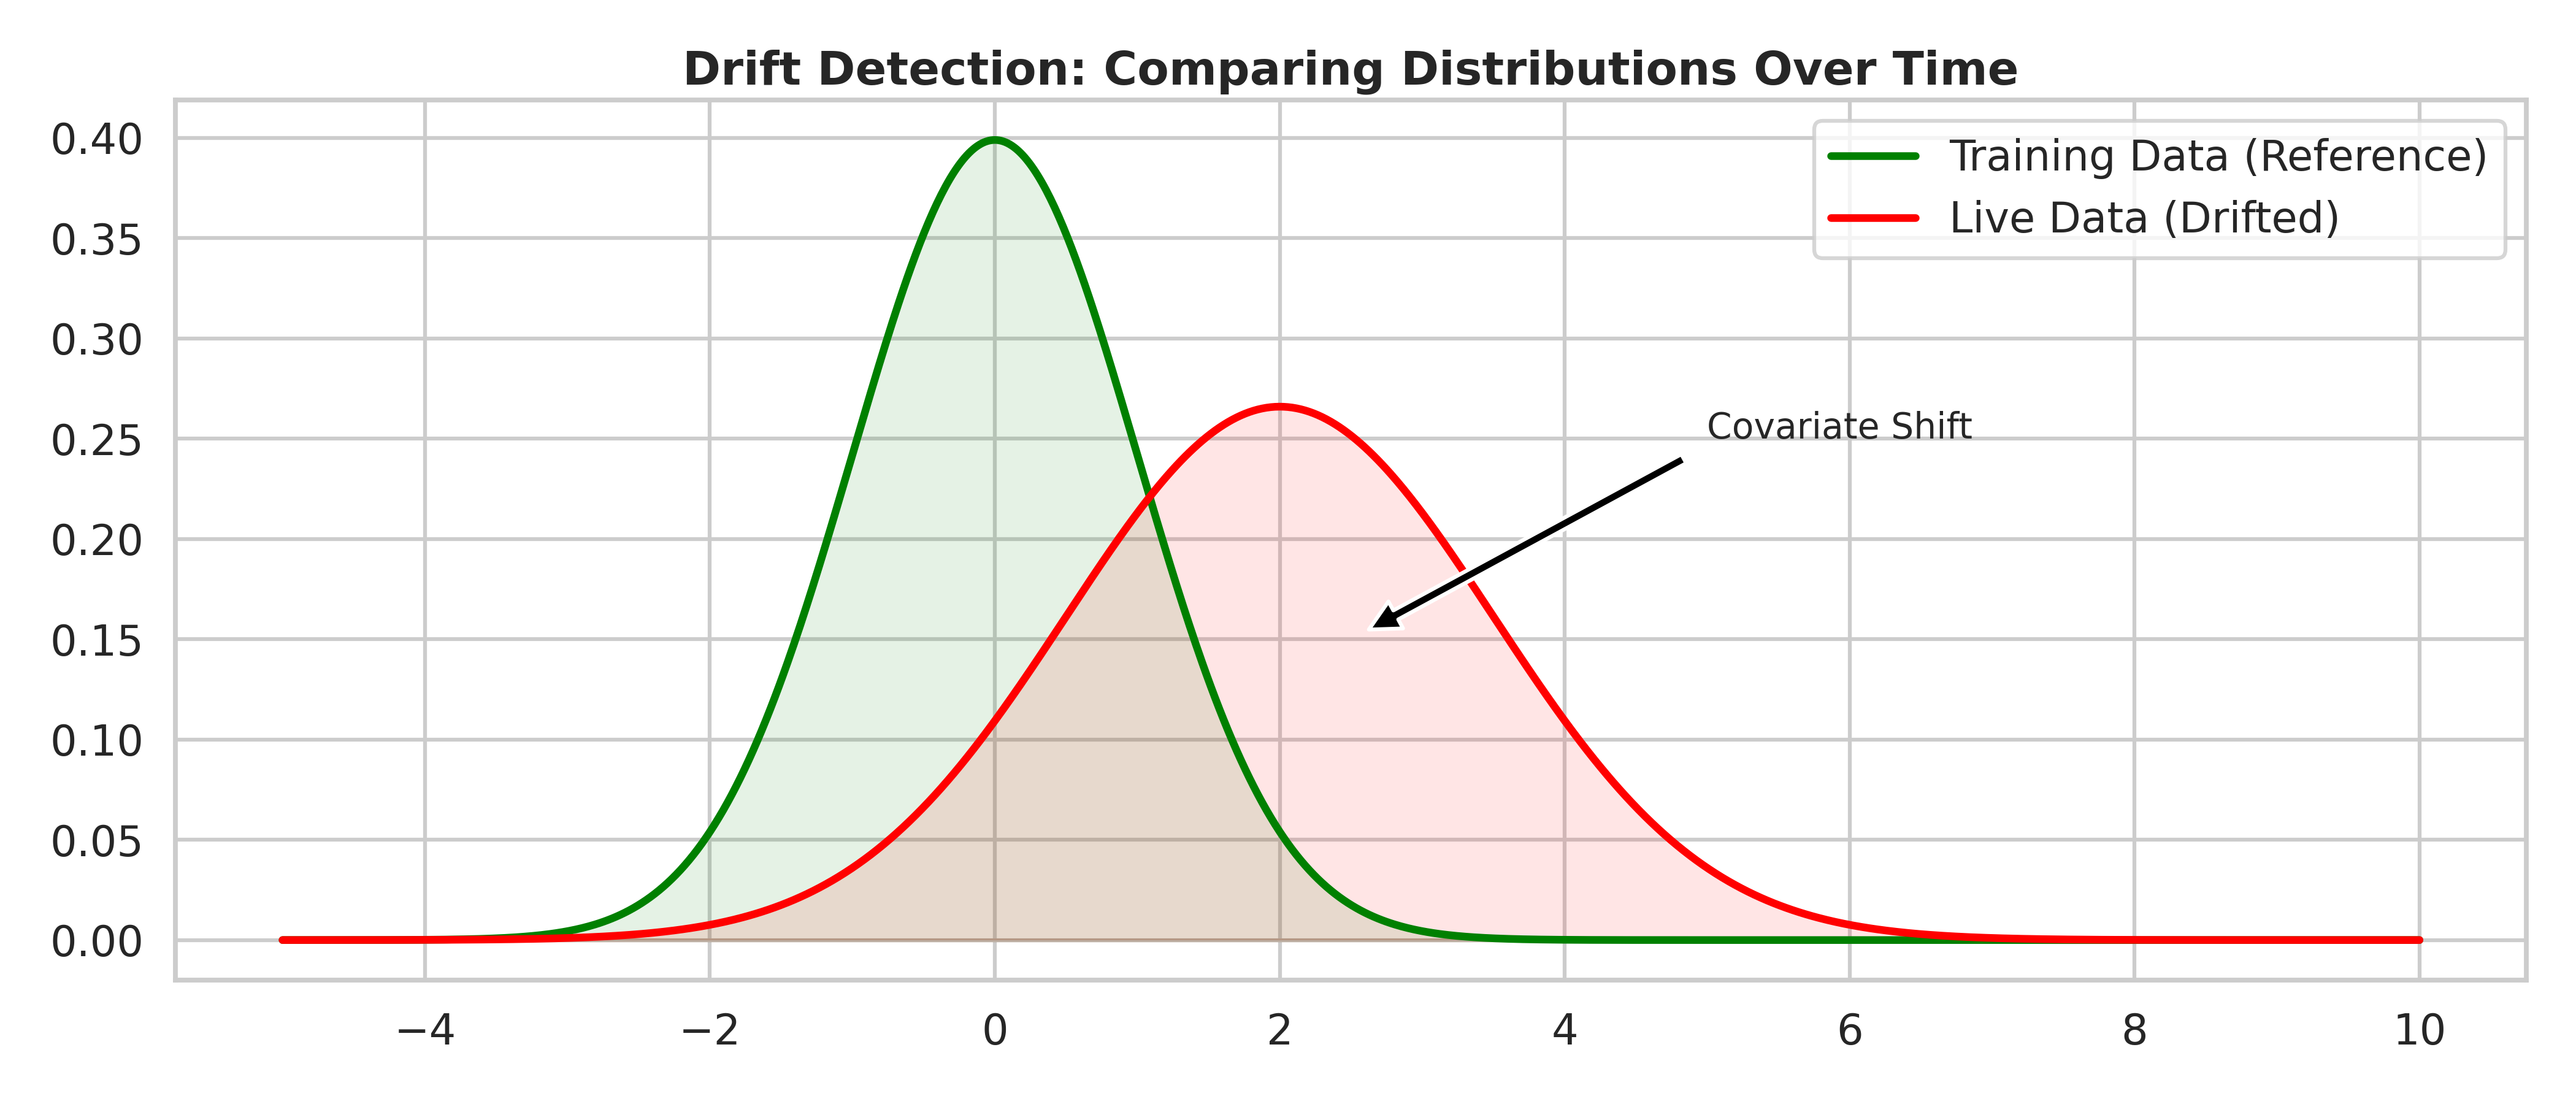
\includegraphics[width=0.95\textwidth]{data_drift.png}
				\caption{\footnotesize KDE overlay of reference and drifted data.}
			\end{figure}
		\end{columns}
		\takeaway{drift detection needs a distance that keeps growing as the live data move away from the reference.}
	\end{frame}

	\begin{frame}{Application 1: A Drift Alarm with $W_1$}
\small
\[
 s_t=W_1(\widehat P_{\mathrm{ref}},\widehat P_t),\qquad
 \mathrm{alarm}_t=\mathbf1\{s_t>\tau\}.
\]
\begin{enumerate}
\item Compare a fixed reference sample with each current window.
\item Calibrate $\tau$ using stable periods with comparable window sizes.
\item Investigate an exceedance before deciding whether to retrain.
\end{enumerate}
\begin{itemize}
\item $W_1$ has the feature's units; a pure translation by $a$ gives $W_1=|a|$.
\item Spread or mode changes require transport too; the score is not generally a mean shift.
\end{itemize}
\end{frame}

	\begin{frame}{Application 2: Wasserstein GANs}
\small
\[
 z\sim P_z\ \xrightarrow{\ G_\theta\ }\ G_\theta(z)\sim P_g,
 \qquad\text{aim: }P_g\approx P_r.
\]
\begin{itemize}
\item Generator: produces samples. Critic: scores real and generated samples.
\item The original minimax GAN objective corresponds to JSD for an optimal discriminator.
\item With little overlap, JSD approaches a plateau.
\item WGAN uses a constrained critic to approximate $W_1$, retaining sensitivity to separation.
\end{itemize}
\end{frame}

	\begin{frame}{WGAN: The Critic Must Be 1-Lipschitz}
\small
For distributions with finite first moments,
\[
 W_1(P_r,P_g)=\sup_{\|f\|_L\le1}\big(\E_{P_r}f-\E_{P_g}f\big),\qquad
 |f(x)-f(y)|\le d(x,y)\quad\forall x,y.
\]
\begin{itemize}
\item Train a neural critic to maximize the score gap under this constraint.
\item Gradient penalty encourages unit gradient norm on sampled interpolants; it is not a global guarantee.
\item Spectral normalization bounds layer amplification; the complete network must respect the Lipschitz bound.
\item A restricted, imperfectly optimized critic approximates the supremum.
\end{itemize}
\end{frame}

	\begin{frame}{Which Measure for Which Job?}
		\small
		\begin{table}[]
			\centering
			\renewcommand{\arraystretch}{1.3}
			\begin{tabular}{l c c l}
				\toprule
				& \textbf{Symmetric} & \textbf{Finite if disjoint} & \textbf{Typical use} \\
				\midrule
				KL $D_{KL}(P\|Q)$ & no & no ($\infty$) & coding, likelihood-based training \\
				JSD & yes & yes (but constant) & overlap checks, simple comparisons \\
				$W_1$ & yes & yes (grows with the gap) & drift detection, generative models \\
				\bottomrule
			\end{tabular}
		\end{table}
		Estimation is the first step: KDE turns samples into densities, and the bandwidth $h$ should be chosen with care before any density-based measure is computed.
		$W_1$ can also be computed directly from samples, without any density estimate.

		\takeaway{choose KL for coding, JSD for simple overlap checks, and Wasserstein when distance between non-overlapping distributions matters.}
	\end{frame}

	% ==============================================================================
	% APPENDIX
	% ==============================================================================
	\appendix
	\sectiondivider{Appendix: optional depth}

	\begin{frame}{Appendix: The AMISE Bandwidth Derivation}
		\small
		\textbf{Scope:} 1-D, second-order kernel, smooth $f$ [Hansen, 2009].
		The \emph{mean integrated squared error} (MISE) is the average, over samples, of $\int(\hat f_h-f)^2dx$.
		For large $n$ and small $h$ it is approximated by the \textbf{AMISE} (``asymptotic'' MISE):
		$$ \text{AMISE}(h) = \underbrace{\frac{R(K)}{nh}}_{\text{variance}} + \underbrace{\tfrac{1}{4} h^4 \mu_2(K)^2 R(f'')}_{\text{squared bias}} $$
		where $R(g)=\int g^2$, $\mu_2(K)=\int u^2K(u)\,du$, and $f''$ is the density curvature.

		\medskip
		Setting $\frac{d}{dh}\text{AMISE}(h) = -\frac{R(K)}{nh^2} + h^3 \mu_2(K)^2 R(f'') = 0$ gives
		$$ h_{\mathrm{opt}} = \left[ \frac{R(K)}{n\,\mu_2(K)^2 R(f'')} \right]^{1/5} \propto n^{-1/5}. $$
		$R(f'')$ is unknown; plugging in a Normal density for $f$ yields Silverman's rule $1.06\,\hat\sigma n^{-1/5}$ for a Gaussian kernel.
	\end{frame}

	\begin{frame}{Appendix: Kernel Order}
		\small
		\textbf{Scope:} second-order kernels, 1-D.
		The \emph{order} of a kernel is the index of its first non-zero moment $\mu_j=\int u^jK(u)\,du$ after $\mu_0=1$.
		Gaussian, Epanechnikov, uniform and triangular kernels are \textbf{second order}: $\mu_1=0$ and $\mu_2(K)>0$.
		The AMISE formula above relies on $\mu_2(K)>0$.

		\medskip
		\emph{Higher-order} kernels have $\mu_2=0$ (and more vanishing moments). They reduce bias faster for very smooth $f$,
		with a different AMISE and a different rate of $h_{\mathrm{opt}}$ in $n$, but they necessarily take negative values,
		so $\hat f_h$ can be negative and is no longer a density.
	\end{frame}

	\begin{frame}{Appendix: Robust Silverman Rule and LSCV}
		\small
		\textbf{Robust rule.} IQR is the 75th minus 25th percentile; for Normal data, $\mathrm{IQR}\approx1.34\sigma$. Use
		$$ h = 0.9\,\min\!\left(\hat\sigma,\ \frac{\mathrm{IQR}}{1.34}\right) n^{-1/5}. $$

		\medskip
		\textbf{Least-squares cross-validation (LSCV).} Choose the $h$ that minimizes
		$$ \mathrm{LSCV}(h)=\int \hat f_h(x)^2\,dx-\frac{2}{n}\sum_{i=1}^n \hat f_{h,-i}(X_i), $$
		where $\hat f_{h,-i}$ is the KDE built \emph{without} sample $X_i$.
		The first term penalizes roughness; the second rewards leave-one-out fit. LSCV avoids the Normal assumption but can be noisy.
	\end{frame}

	\begin{frame}{Appendix: Marginal Constraints of the Transport Plan}
		\small
		The set $\Pi(P,Q)$ of allowed plans consists of the $\gamma(x,y)\ge 0$ with the correct marginals:
		$$ \int \gamma(x, y)\, dy = p(x) \quad \text{(all mass at } x \text{ is shipped out)}, $$
		$$ \int \gamma(x, y)\, dx = q(y) \quad \text{(all mass at } y \text{ is delivered)}. $$
		We can neither create nor destroy mass, only move it.
	\end{frame}

	\begin{frame}{Appendix: Discrete Wasserstein as a Linear Program}
		\small
		For samples, put weights $\mathbf a\in\Delta_n$ at points $x_i$ and $\mathbf b\in\Delta_m$ at points $y_j$,
		where $\Delta_n$ is the \emph{probability simplex}: vectors with non-negative entries that sum to 1.
		The cost matrix is $C_{ij}=d(x_i,y_j)^p$, and the plan is a matrix $\Gamma\in\R^{n\times m}$, $\Gamma_{ij}$ being the mass moved from $x_i$ to $y_j$.

		\begin{block}{Kantorovich linear program}
			$$ \Gamma^* = \argmin_{\Gamma\ge 0} \sum_{i,j} C_{ij}\Gamma_{ij}
				\quad\text{subject to}\quad \Gamma \mathbf{1}_m = \mathbf{a},\ \ \Gamma^{\top} \mathbf{1}_n = \mathbf{b}. $$
		\end{block}
		The two constraints are the discrete marginal conditions (row sums give $\mathbf a$, column sums give $\mathbf b$).
		The minimum value is $W_p^p$. Example metrics: $d(x,y)=\|x-y\|_1$ or $\|x-y\|_2$.
	\end{frame}

	\begin{frame}{Appendix: The Kantorovich--Rubinstein Dual and WGAN}
		\small
		For $p=1$, the Wasserstein distance has the dual form
		$$ W_1(P_r, P_g) = \sup_{\|f\|_L \le 1} \ \E_{x \sim P_r}[f(x)] - \E_{x \sim P_g}[f(x)], $$
		with the \textbf{1-Lipschitz} constraint $|f(x)-f(y)|\le d(x,y)$ for all $x,y$.
		A neural critic $f_w$ approximates the maximizer.

		\begin{itemize}
			\item \textbf{Gradient penalty:} add $\lambda\,\E_{\hat x}\big[(\|\nabla_{\hat x} f_w(\hat x)\|_2-1)^2\big]$ to the critic loss, with $\hat x$ sampled between real and generated points.
			\item \textbf{Spectral normalization:} divide each weight matrix by its largest singular value; for 1-Lipschitz activations the network is then 1-Lipschitz.
		\end{itemize}
	\end{frame}

\end{document}
